\scanpage{61}
% block: reconstruction continued
$\handwritten{\mathcal{M}}$ in terms of the \unsure{family|family} of the $A_i$ \deleted{and of the integers $d_i=\operatorname{rang}E_i$} as follows\deleted{e}. One first considers the preadditive categories \deleted{generated} having as objects the elements $\handwritten{\underline{\unsure{Y|\gamma}}}$ of $\underline{N}^{(I)}$, ($\handwritten{\underline{\gamma}}=(\handwritten{\gamma}_i)_{i\handwritten{\in}I}$ being interpreted as $\handwritten{\bigotimes}E_i^{\handwritten{\gamma}_i}$), \deleted{or} with $\operatorname{Hom}(\handwritten{\underline{\gamma}},\handwritten{\underline{\gamma}'})=0$ if $\handwritten{\underline{\gamma}\ne\underline{\gamma}'}$ and $=\bigotimes_{\handwritten{i}} A_i^{\otimes\handwritten{\gamma_i}}$ if $\handwritten{\underline{\gamma}=\underline{\gamma}'}$, the composition of morphisms obvious. One defines in the obvious way the functor $\otimes$ (addition of $\underline{N}^{(I)}$ on objects, tensor product on homomorphisms) and its constra\unsure{int}s,\margin{\handwritten{\unsure{attention to} commutativity constraint}} so that one finds a sub-$\otimes$-category. Its Karoubian envelope is an abelian \inserted{$\otimes$-\begin{tikzpicture}[x=1cm,y=1cm,baseline=-.1cm]\draw[thin] (0,.2).. controls (-.3,-.1) and (-.85,.1)..(-1.05,-.16).. controls (-1.2,-.3) and (-1.25,-.4)..(-1.15,-.55);\end{tikzpicture}}category, which is identified with the full subcategory of $\handwritten{\mathcal{M}}$ consisting of the elements whose nonzero homogeneous components are in degrees $\handwritten{\in}\underline{N}^{(I)}$,\inserted{and has a fibre functor over \deleted{$k$}
\begin{tikzpicture}[x=1cm,y=1cm,baseline=-.1cm]\draw[thin] (0,.3).. controls (-.1,-.05) and (-.2,-.1)..(-1,-.06)--(-4.6,.03).. controls (-4.95,.03) and (-5,.03)..(-5,-.4);\draw[thin] (-.45,.35)--(-.55,.02).. controls (-.8,-.2) and (-.7,-.3)..(-.65,-.1)--(-.45,.35);\end{tikzpicture}}\margin{\figure{\begin{tikzpicture}[x=1cm,y=1cm]\node at (.6,.3) {$\overset{\handwritten{-}}{k}$.};\draw[thin] (.6,.3) ellipse (.63 and .47);\draw[thin] (-.05,.5)--(-.17,-.12).. controls (-.43,-.45) and (-.31,-.48)..(-.25,-.24)--(-.05,.5);\end{tikzpicture}}} On the other hand, for every $i$, if $A_i$ is of \deleted{degree}\inserted{rank} $d_i^2$ (thus $E_i$ of rank $d_i$), let $L_i=\det E_i={\handwritten{\unsure{A|\bigwedge}_{\unsure{t|2|k}}}}^{d_i}\handwritten{E_i}$ (where $E_i$ denotes the object of the constructed category corresponding \deleted{to \unsure{the|it|the}} $i$.th element of the canonical basis of $\underline{Z}^{(I)}$, namely $\unsure{1|l}_i$ ...), it is a pre-invertible object ($\inserted{\handwritten{X\to\begin{tikzpicture}[x=1cm,y=1cm,baseline=-.1cm]\draw[thin] (0,.2).. controls (-.3,-.1) and (-.85,.1)..(-1.05,-.16).. controls (-1.2,-.3) and (-1.25,-.4)..(-1.15,-.55);\end{tikzpicture}}}\deleted{\unsure{\otimes}}L_i\otimes\handwritten{X}$ is fully faithful) and by inverting the $L_i$, one finds (up to \deleted{equ}equivalence\deleted{)} respecting everything) the category $\handwritten{\mathcal{M}}$.

% block: nonfree case
When $\handwritten{\unsure{\Gamma|T}}$ is not free, one finds an analogous construction in terms of a \inserted{suitable\begin{tikzpicture}[x=1cm,y=1cm,baseline=-.1cm]\draw[thin] (0,.2).. controls (-.3,-.1) and (-.85,.1)..(-1.05,-.16).. controls (-1.2,-.3) and (-1.25,-.4)..(-1.15,-.55);\end{tikzpicture}} system of generators $(\handwritten{\gamma}_i)_{i\handwritten{\in}I}$, but by``ren\unsure{d|a}ering \deleted{in addition} equal to 1 \unsure{\deleted{x}|$^{x}$}'' certain further elements.\margin{To be made explicit !} These constructions are well suited for describing the $\otimes$-functors from $\handwritten{\mathcal{M}}$ into a Tannakian \deleted{$\otimes$-}category, and for describing base change.( For this last reason in particular, it would have been awkward in the general case to take the $\unsure{\mathbb{M}|M}_i$ simple ....). Take care, in the description of the $\otimes$-functors in question, to take account of the c\deleted{d}onstraints, in particular of that o\deleted{\unsure{i}}f commutativity; it seems that it should come to the same thing to require that the rank is preserved ...
% archive sheet number: 60
